\documentclass[]{article}
\usepackage{graphicx}
\graphicspath{{figs/}} 
%opening
\title{Notes from Origins of Life}
\author{}

\begin{document}

\maketitle


\begin{abstract}
    This course aims to push the field of Origins of Life research forward by bringing new and synthetic thinking to the question of how life emerged from an abiotic world.

This course begins by examining the chemical, geological, physical, and biological principles that give us insight into origins of life research. We look at the chemical and geological environment of early Earth from the perspective of likely environments for life to originate.

Taking a look at modern life we ask what it can tell us about the origin of life by winding the clock backwards. We explore what elements of modern life are absolutely essential for life, and ask what is arbitrary? We ponder how life arose from the huge chemical space and what this early 'living chemistry' may have looked like.

We examine phenomena, that may seem particularly life like, but are in fact likely to arise given physical dynamics alone. We analyze what physical concepts and laws bound the possibilities for life and its formation.

Insights gained from modern evolutionary theory will be applied to proto-life. Once life emerges, we consider how living systems impact the geosphere and evolve complexity. 

The study of Origins of Life is highly interdisciplinary - touching on concepts and principles from earth science, biology, chemistry, and physics.  With this we hope that the course can bring students interested in a broad range of fields to explore how life originated. 

The course will make use of basic algebra, chemistry, and biology but potentially difficult topics will be reviewed, and help is available in the course discussion forum and instructor email. There will be pointers to additional resources for those who want to dig deeper.

This course is Complexity Explorer's first Frontiers Course.  A Frontiers Course gives students a tour of an active interdisciplinary research area. The goals of a Frontiers Course are to share the excitement and uncertainty of a scientific area, inspire curiosity, and possibly draw new people into the research community who can help this research area take shape!

\end{abstract}

\tableofcontents
\listoffigures

\section{Introduction}
\subsection{Welcome To The Course}
\subsection{Life}
\cite{bell2015potentially}
\subsection{Nonequilibrium Physics}
\subsection{Constraining Chemical Complexity to Form Life}
\subsection{Geological Conditions, Change, and Chaos}
\subsection{Pattern Formation in Chemical Systems}
\subsection{The Central Dogma of Biology}
\cite{crick1958biological} \cite{crick1970central}
\subsection{Biological Similarity}
\subsection{Selection Theory}
\cite{eigen1978hypercycle} \cite{eigen1988molecular} \cite{eigen2002error} \cite{crotty2001rna} \cite{stadtler2002fitness_landscapes}
\section{Chemical Origins}
\subsection{Introduction}

We will discuss likely chemistry of the early Earth, chemistry that may be to be fundamental to the origin of life, what we know is essential for biochemistry of modern life, processes that can occur in chemical dynamics, and extreme life that occurs today in a variety of environments.


\subsection{What Did Early Earth Look Like?}

\subsubsection{Geochemical Landscape}
\begin{figure}[h!]
	\caption{Geochemical Landscape after \cite{kitadai2018origins}}
	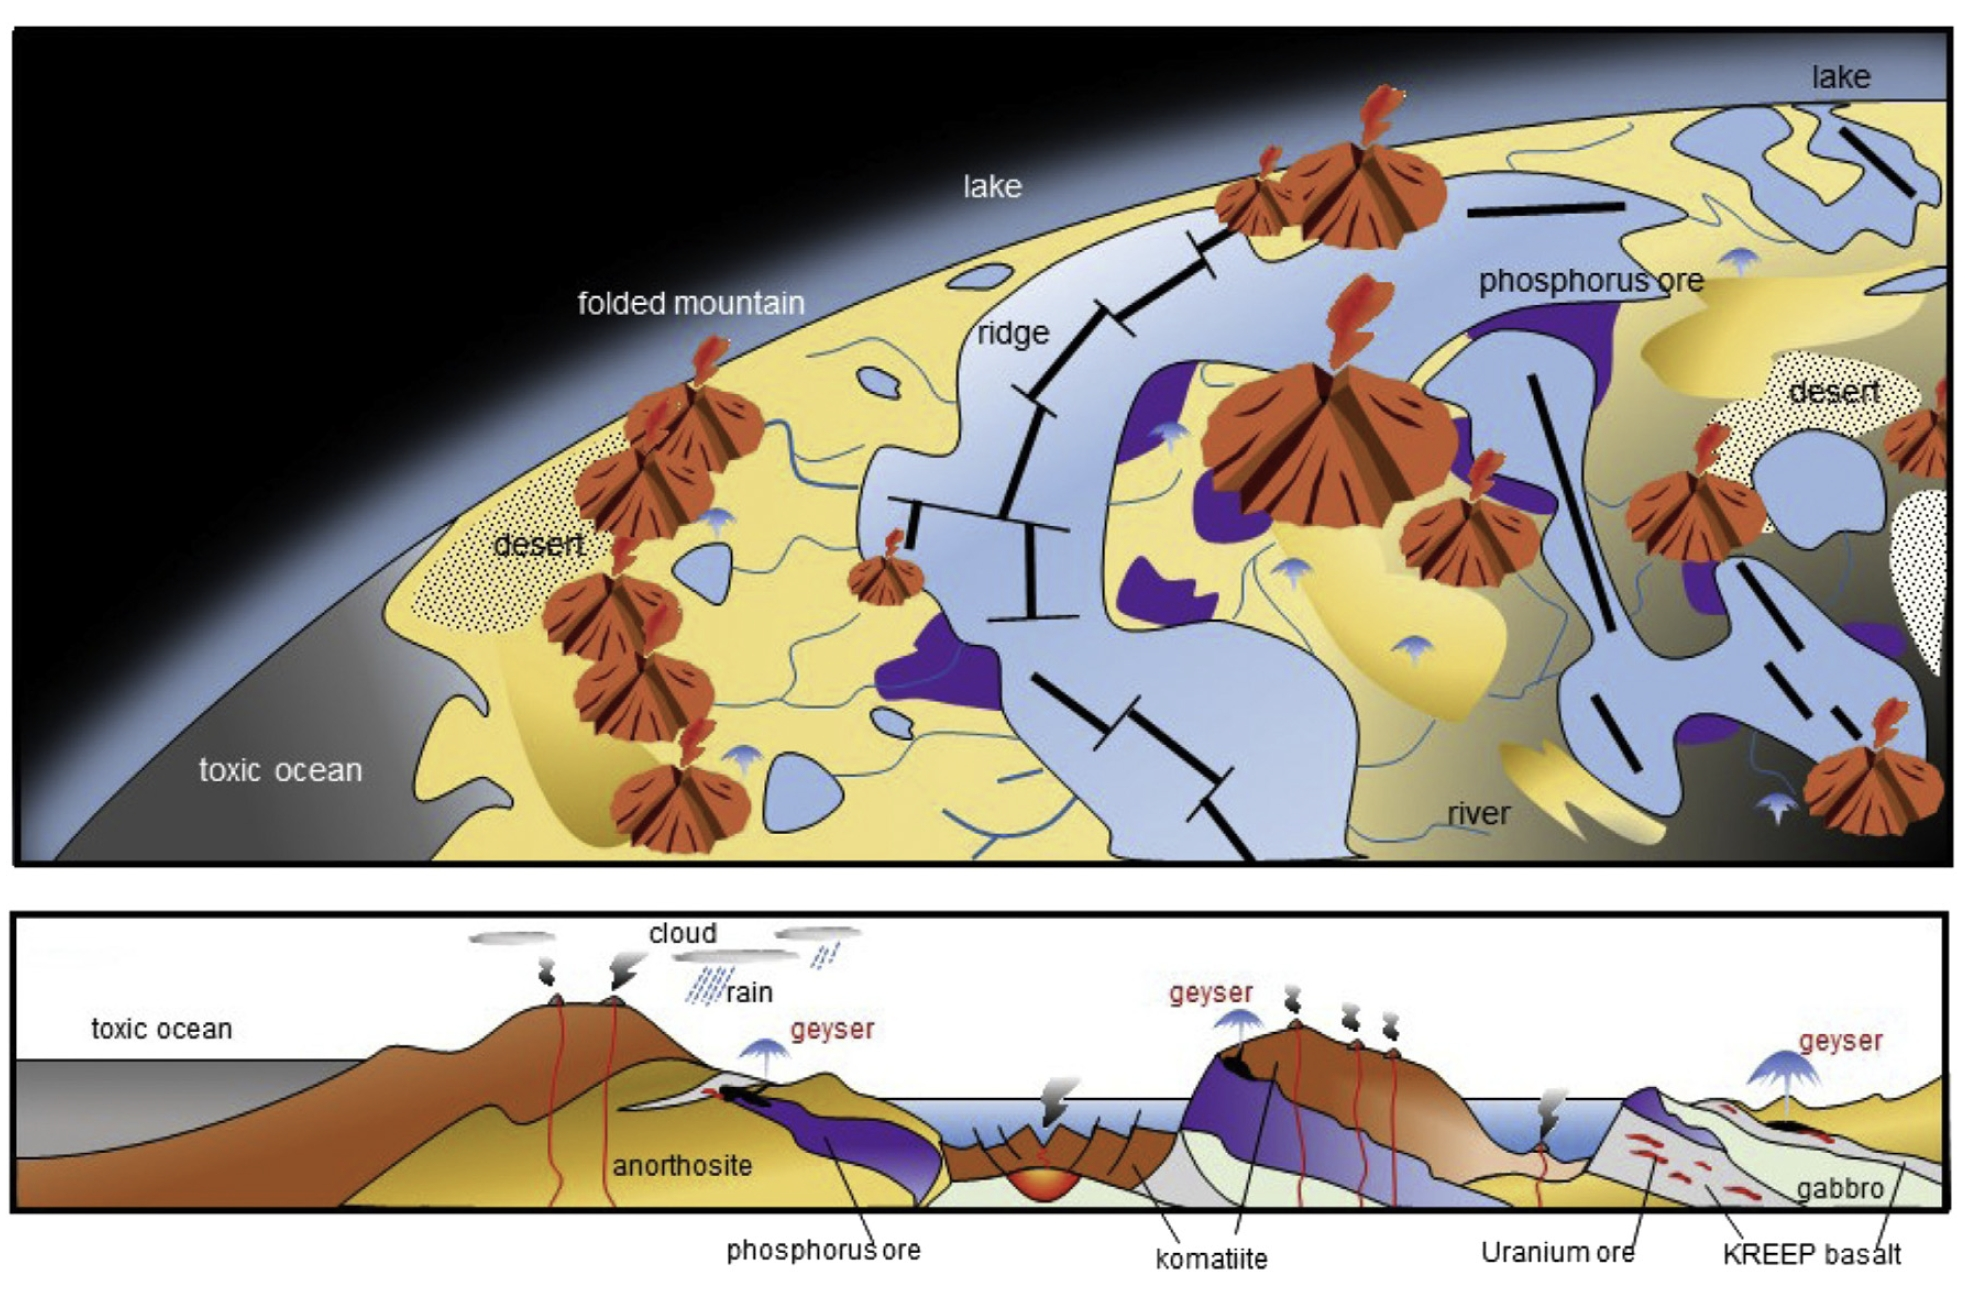
\includegraphics[width=0.9\textwidth]{GeochemicalLandscape}
\end{figure}

  
  \begin{itemize}
  	\item  Definitely an ocean that was warmer than today, probably saltier.
  	\item Landmasses from volcanic activity, and, maybe, plate tectonics.
  	\item On continents, lakes and ponds from precipitation.  Maybe temporary streams from precipitation.
  	\item Surfaces composed of minerals, which were good for catalysis and energy production. Today covered with life.
  \end{itemize}


\subsubsection{Mixing processes between chemical reactors}
\begin{figure}[h!]
	\caption{Mixing processes between chemical reactors \cite{stueken2013did}}
	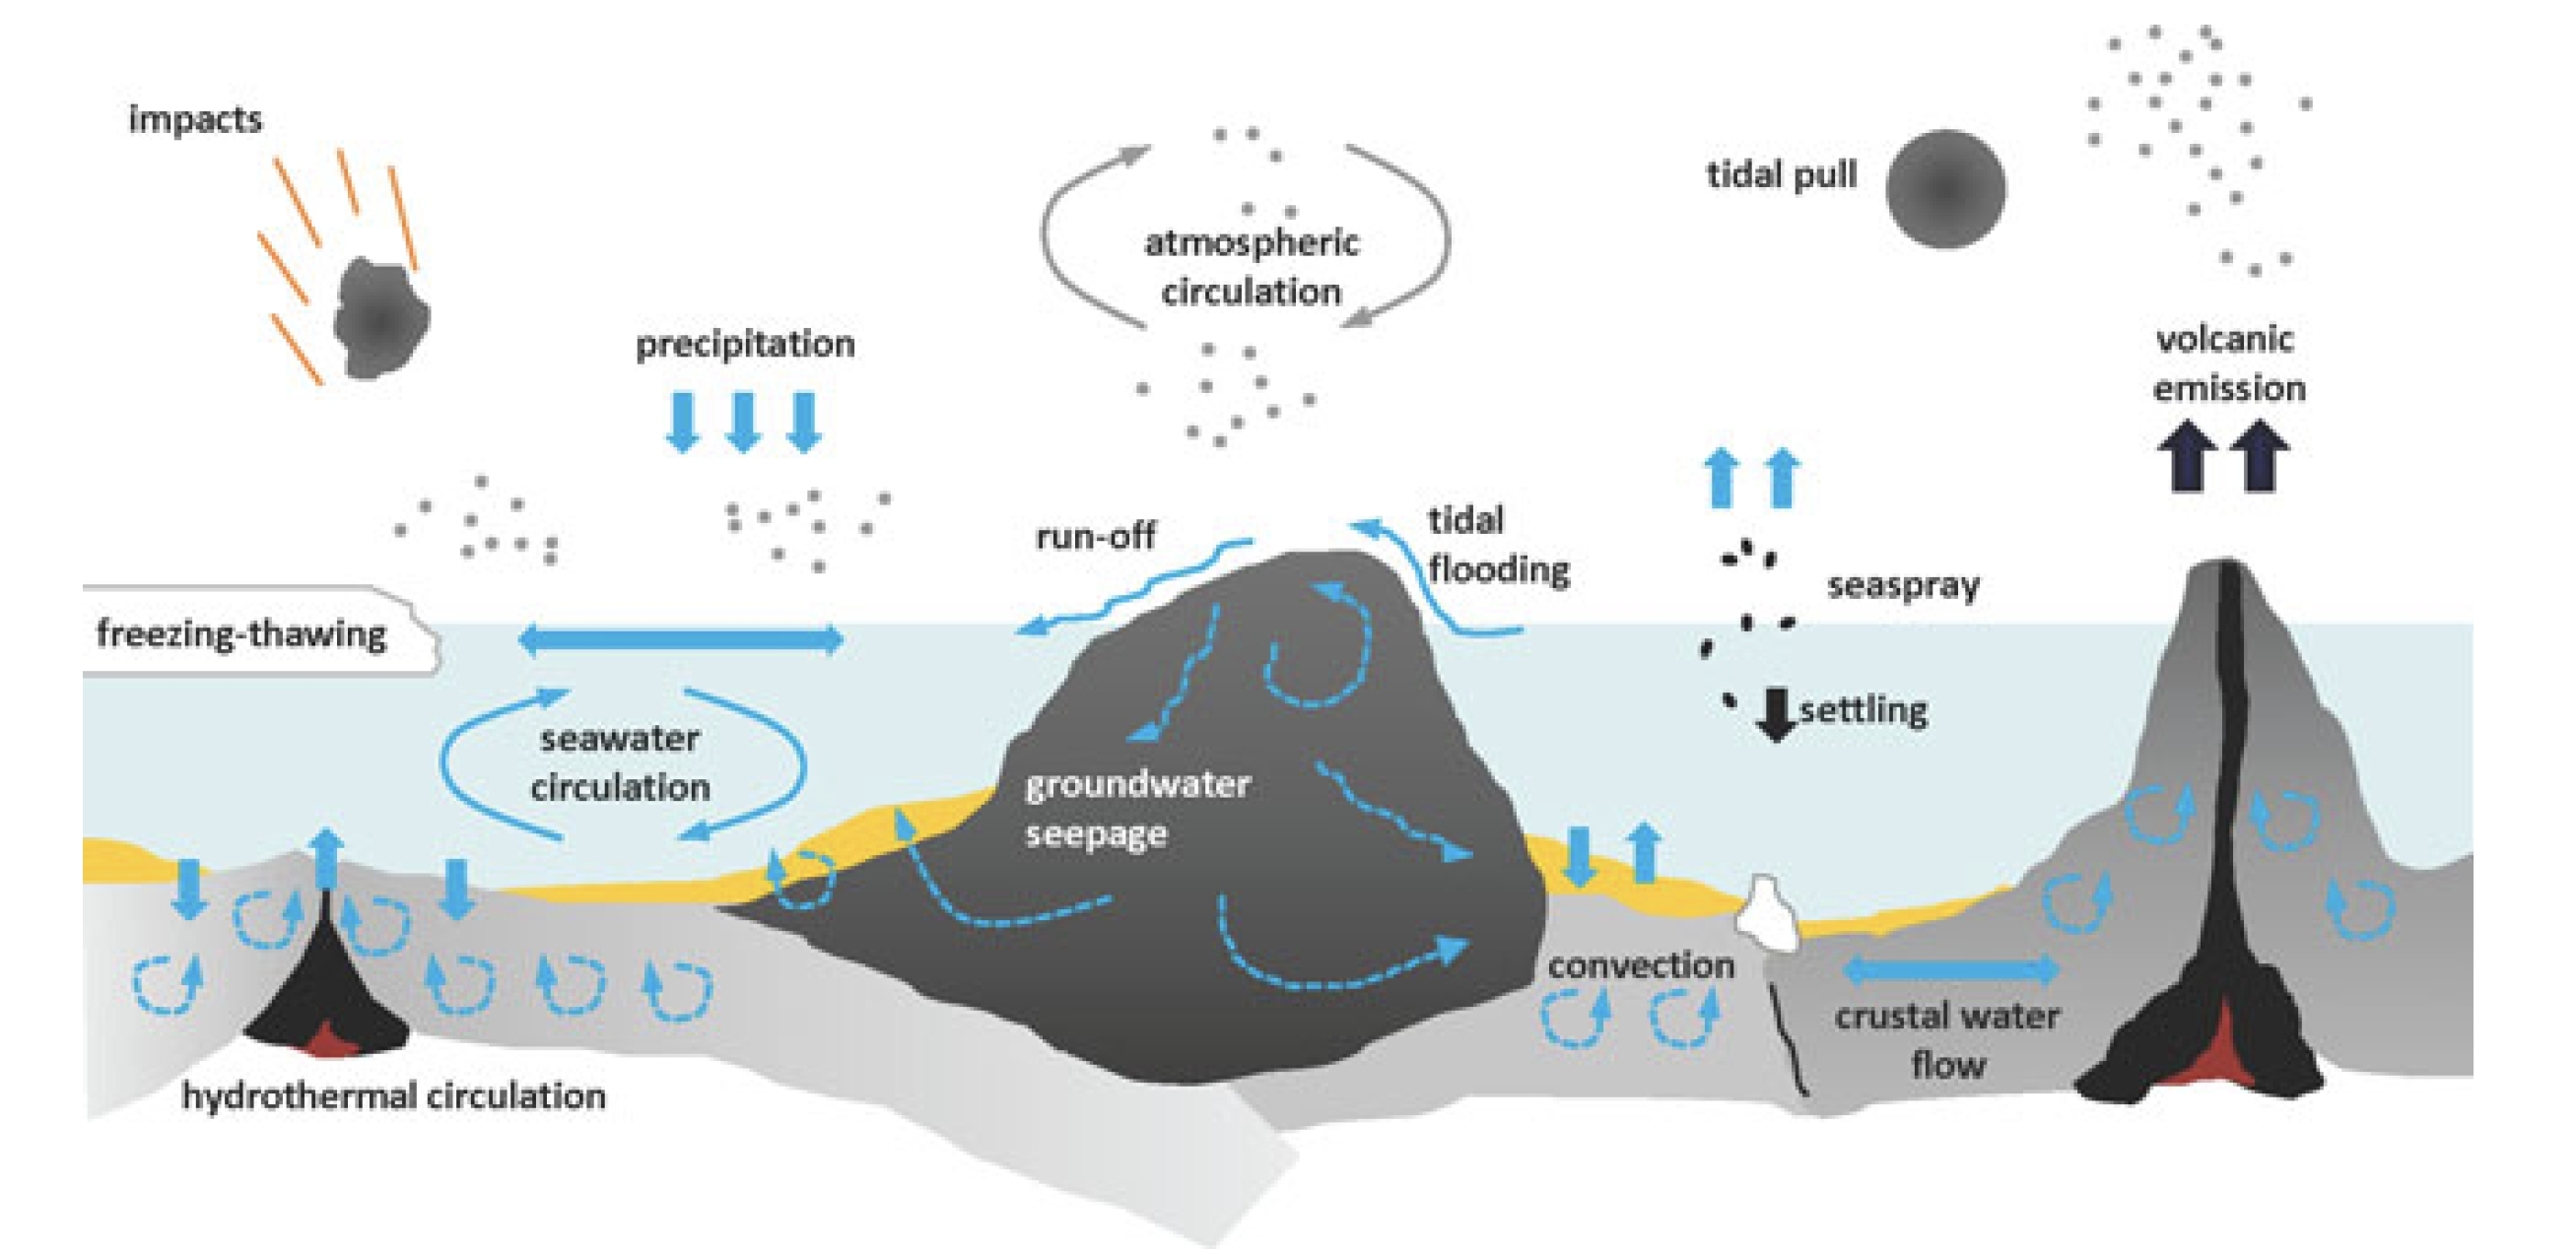
\includegraphics[width=0.9\textwidth]{MixingProcesses}
\end{figure}
Chemical reactions mixed by a variety of processes.

\begin{itemize}
	\item Tides
	\item Evaporation and aerosols
	\item Volcanic plumes
	\item Hydrothermal vents
\end{itemize}
  
  
\subsubsection{Mixing processes between chemical reactors}
Reactions would have been mixed by different processes.\cite{stueken2013did}
\subsection{Likely Environments for Studying Origins of Life}
\subsection{Chemistry and The Origins of Life}
\subsection{Why Nature Chose Phosphates}
\subsection{Why Water, Why Carbon}
\subsection{Macromolecules}
\subsection{Chemical Cycles and Chaos}
\subsection{Fossil or Not?}

\section{Chemical Commonalities}

\section{Early Life}

\section{Evolution}

\section{Astrobiology \& General Theories of Life}

\bibliographystyle{unsrt}
\bibliography{origins}

\end{document}
